% Apresentação de progresso, 02/12/2026: metodologia e resultados do estudo de kernels (artigo report/artigo_kernel/).
% Público: conhece redes neurais e hardware, não as arquiteturas específicas. 14 páginas (12 da de julho + figuras pedidas).
% Números: report/artigo_kernel/artigo_kernel.tex e results/phase_13_*/all_runs.csv.
% Figuras lidas direto de results/figures_generated/ (sem cópias); trims iguais aos do artigo.
% Build: latexmk -pdf slides.tex
\documentclass[t,aspectratio=169,12pt,xcolor=table]{beamer}
\usepackage{booktabs}
\usepackage{tikz}
\usetikzlibrary{positioning}

\definecolor{fundo}{HTML}{FFF8E1}
\definecolor{ardosia}{HTML}{455A64}
\definecolor{linha}{HTML}{EDE6D3}
\setbeamercolor{background canvas}{bg=fundo}
\setbeamercolor{normal text}{fg=ardosia}
\setbeamercolor{frametitle}{fg=ardosia}
\setbeamercolor{title}{fg=ardosia}
\setbeamercolor{subtitle}{fg=ardosia}
\setbeamercolor{itemize item}{fg=ardosia}
\setbeamercolor{bibliography entry author}{fg=ardosia}
\setbeamercolor{bibliography entry title}{fg=ardosia}
\setbeamercolor{bibliography entry note}{fg=ardosia}
\setbeamerfont{frametitle}{series=\bfseries,size=\LARGE}
\setbeamerfont{title}{series=\bfseries,size=\huge}
\setbeamertemplate{navigation symbols}{}
\setbeamertemplate{itemize item}{\textbullet}
\setbeamertemplate{bibliography item}{[\theenumiv]}
\setbeamertemplate{footline}{\hfill\insertframenumber\hspace{1.2em}\vspace{0.8em}}
\setbeamertemplate{frametitle}{\vspace{0.6em}\insertframetitle\vspace{0.2em}}

\graphicspath{{../../results/figures_generated/}}
\renewcommand{\arraystretch}{1.45}
\setlength{\tabcolsep}{8pt}
\newcommand{\by}{\texttimes}
\newcommand{\cab}{\rowcolor{ardosia}}          % cabeçalho de tabela em ardósia
\newcommand{\bc}[1]{\textcolor{white}{\textbf{#1}}}
\newcommand{\nota}[1]{\par\vspace{0.4em}{\small\itshape #1}}

\title{Restrição do Tamanho de Kernel em CNNs e Sua Eficiência}
\subtitle{Apresentação de progresso}
\author{Rafael Silva de Souza}
\date{2 de dezembro de 2026}

\begin{document}

\begin{frame}[plain]
  \centering\vfill
  {\usebeamerfont{title}\usebeamercolor[fg]{title}\inserttitle\par}
  \vspace{0.8em}{\Large\insertsubtitle\par}
  \vfill
  {\large\insertauthor\par}\vspace{0.3em}\insertdate
  \vspace{1.5em}
\end{frame}

\begin{frame}{Motivação}
  \begin{itemize}\setlength{\itemsep}{0.7em}
    \item As convoluções são quase todo o custo de uma CNN
    \item A convolução Winograd~\cite{lavin} troca multiplicações por somas, e os aceleradores costumam ser feitos para um kernel pequeno (3\by3, 2\by2)
    \item Kernels grandes (5\by5, 11\by11) ficam de fora do acelerador
  \end{itemize}
  \bigskip
  \textbf{Pergunta:} se todos os kernels forem 3\by3 ou 2\by2, quanto se perde de acurácia? Dá para recuperar mudando o resto da rede? O resultado sobrevive a INT8 e à aritmética do acelerador?
\end{frame}

\begin{frame}{O Que Varia Numa CNN}
  \centering
  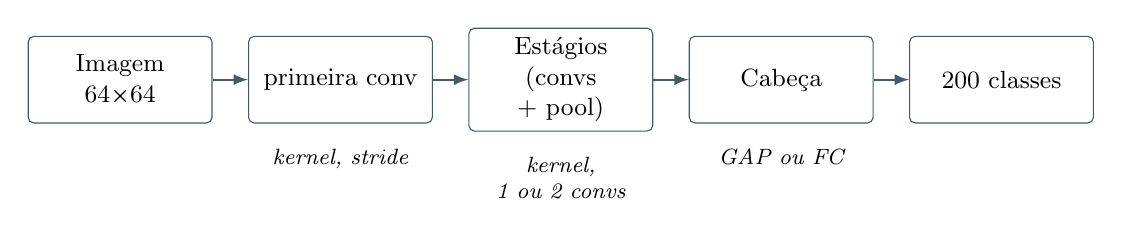
\begin{tikzpicture}[node distance=0.45cm, >=latex,
      bloco/.style={draw=ardosia, fill=white, rounded corners=2pt, align=center,
                    minimum height=1.1cm, text width=2.1cm, font=\small},
      fator/.style={align=center, text width=2.3cm, font=\footnotesize\itshape}]
    \node[bloco] (in) {Imagem\\64\by64};
    \node[bloco, right=of in] (c1) {primeira conv};
    \node[bloco, right=of c1] (st) {Estágios\\(convs + pool)};
    \node[bloco, right=of st] (hd) {Cabeça};
    \node[bloco, right=of hd] (out) {200 classes};
    \draw[->, ardosia, thick] (in) -- (c1);
    \draw[->, ardosia, thick] (c1) -- (st);
    \draw[->, ardosia, thick] (st) -- (hd);
    \draw[->, ardosia, thick] (hd) -- (out);
    \node[fator, below=0.2cm of c1] {kernel, stride};
    \node[fator, below=0.2cm of st] {kernel,\\1 ou 2 convs};
    \node[fator, below=0.2cm of hd] {GAP ou FC};
  \end{tikzpicture}
  \raggedright\small
  \begin{itemize}\setlength{\itemsep}{0.15em}
    \item \textbf{Kernel:} tamanho do filtro (k\by k), o que o acelerador restringe
    \item \textbf{Stride:} passo da conv; stride 4 reduz a imagem 4\by\ logo na entrada
    \item \textbf{Estágio:} convs na mesma resolução, entre dois poolings
    \item \textbf{Cabeça FC:} achata o mapa final e usa camadas densas (muitos parâmetros); \textbf{GAP:} média de cada canal e uma camada linear
    \item \textbf{BN:} normaliza as ativações de cada canal; estabiliza o treino
  \end{itemize}
\end{frame}

\begin{frame}{As Redes}
  \begin{center}\small
  \begin{tabular}{l >{\raggedright\arraybackslash}p{0.58\textwidth} c}
    \cab \bc{Rede} & \bc{Ideia} & \bc{Kernels} \\
    AlexNet~\cite{alexnet} & 5 convs; a primeira grande, com stride 4; cabeça FC grande & 11-5-3-3-3 \\
    \rowcolor{linha}
    VGG16~\cite{vgg} & 13 convs pequenas empilhadas em 5 estágios & 3\by3 \\
    ResNet-18~\cite{resnet} & blocos com atalho: a entrada é somada à saída & 7\by7 e 3\by3 \\
    \rowcolor{linha}
    Fire~\cite{squeezenet} & conv 1\by1 reduz os canais antes da 3\by3: $\sim$4\by\ menos parâmetros & 1\by1 e 3\by3 \\
  \end{tabular}
  \end{center}
  \nota{Restringir o kernel = trocar todos por 3\by3 ou 2\by2 e manter o resto. Todas adaptadas a imagens 64\by64.}
\end{frame}

\begin{frame}{Metodologia: Experimento}
  \begin{itemize}\setlength{\itemsep}{0.35em}
    \item \textbf{Dados:} Tiny ImageNet~\cite{tiny}: 100 mil imagens 64\by64, 200 classes; top-1 em 10 mil imagens de teste
    \item \textbf{Um fator por vez:} pares de redes iguais exceto num fator (kernel, cabeça, stride\ldots)
    \item \textbf{Mesma receita para todas:} SGD (gradiente descendente estocástico) com momentum, sem parada antecipada
    \item \textbf{Ruído:} o mesmo treino com 3 sementes varia $\pm$0,8 p.p.; diferença menor é empate. 338 treinos ao todo
  \end{itemize}
  \medskip
  \centering
  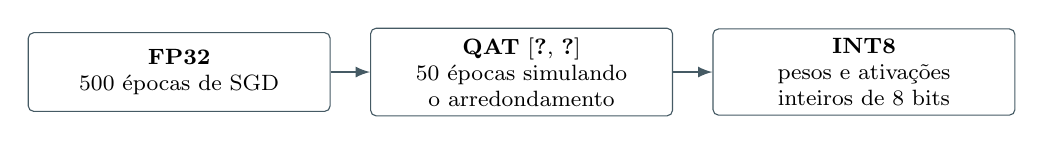
\begin{tikzpicture}[node distance=0.5cm, >=latex,
      etapa/.style={draw=ardosia, fill=white, rounded corners=2pt, align=center,
                    minimum height=1.0cm, text width=3.6cm, font=\footnotesize}]
    \node[etapa] (fp) {\textbf{FP32}\\500 épocas de SGD};
    \node[etapa, right=of fp] (qat) {\textbf{QAT}~\cite{jacob,wu}\\50 épocas simulando\\o arredondamento};
    \node[etapa, right=of qat] (int8) {\textbf{INT8}\\pesos e ativações inteiros de 8 bits};
    \draw[->, ardosia, thick] (fp) -- (qat);
    \draw[->, ardosia, thick] (qat) -- (int8);
  \end{tikzpicture}
\end{frame}

\begin{frame}{Metodologia: Convolução Winograd}
  \centering
  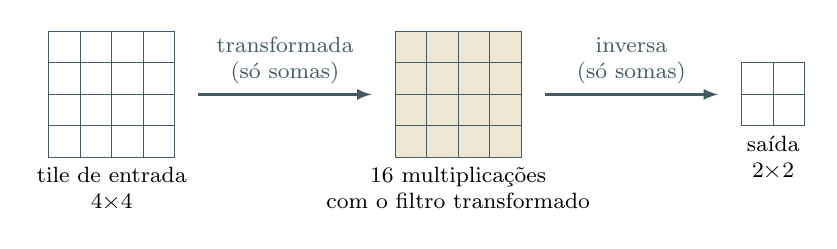
\begin{tikzpicture}[>=latex, font=\footnotesize]
    \filldraw[fill=white, draw=ardosia] (0,0) rectangle (1.6,1.6);
    \draw[ardosia, step=0.4] (0,0) grid (1.6,1.6);
    \node[align=center, below] at (0.8,0) {tile de entrada\\4\by4};
    \draw[->, ardosia, thick] (1.9,0.8) -- node[above, align=center] {transformada\\(só somas)} (4.1,0.8);
    \filldraw[fill=linha, draw=ardosia] (4.4,0) rectangle (6.0,1.6);
    \draw[ardosia, step=0.4] (4.4,0) grid (6.0,1.6);
    \node[align=center, below] at (5.2,0) {16 multiplicações\\com o filtro transformado};
    \draw[->, ardosia, thick] (6.3,0.8) -- node[above, align=center] {inversa\\(só somas)} (8.5,0.8);
    \filldraw[fill=white, draw=ardosia] (8.8,0.4) rectangle (9.6,1.2);
    \draw[ardosia, step=0.4] (8.8,0.4) grid (9.6,1.2);
    \node[align=center, below] at (9.2,0.4) {saída\\2\by2};
  \end{tikzpicture}
  \par\medskip
  {\small F(2\by2, 3\by3): 16 multiplicações onde a conv direta faz 4 \by\ 9 = 36~\cite{lavin}}
  \raggedright
  \begin{itemize}\setlength{\itemsep}{0.35em}
    \item Tiles maiores economizam mais (F(4,3): 4\by; F(6,3): 5,1\by), mas as transformadas amplificam o erro numérico~\cite{barabasz}
    \item Simulamos a aritmética de ponto fixo do acelerador Winograd em FPGA do grupo~\cite{schmitz} durante o QAT, em 16 redes
  \end{itemize}
\end{frame}

\begin{frame}{O Custo do Kernel Depende da Cabeça}
  \begin{center}\small
  \begin{tabular}{lccc}
    \cab \bc{Kernels} & \bc{Top-1 com GAP} & \bc{Top-1 com FC} & \bc{MACs das convs} \\
    11-5-3-3-3 (AlexNet) & 53,1\,\% & 52,2\,\% & 240M \\
    \rowcolor{linha}
    3\by3 & 53,8\,\% & 50,7\,\% & 167M \\
    2\by2 & 52,6\,\% & 45,7\,\% & 75M \\
  \end{tabular}
  \end{center}
  \begin{itemize}\setlength{\itemsep}{0.3em}
    \item \textbf{GAP:} 2\by2 perde só 0,5 p.p.\ com 69\,\% menos MACs
    \item \textbf{FC:} 2\by2 perde 6,6 p.p.
    \item VGG16 e ResNet-18 com GAP: 3\by3 $\rightarrow$ 2\by2 custa 1,0--2,4 p.p.
  \end{itemize}
\end{frame}

\begin{frame}{Kernel ou Capacidade?}
  \centering
  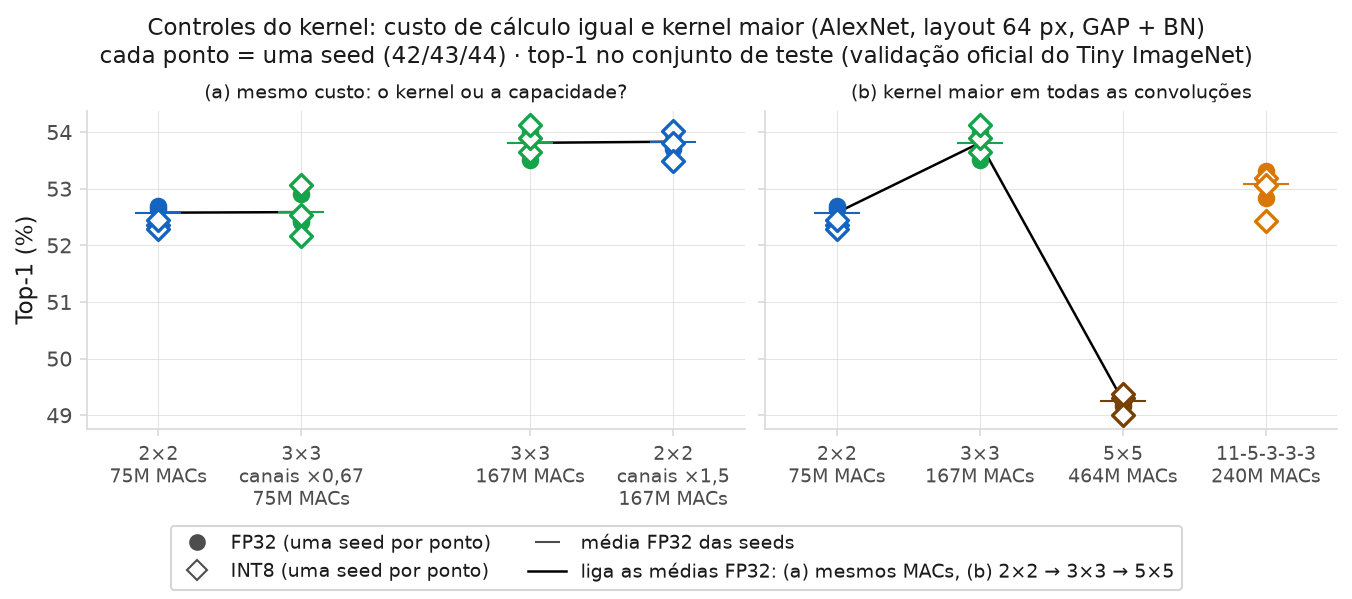
\includegraphics[width=0.92\textwidth,trim=0 0 0 36,clip]{phase_11_kernel_size_comparison/26_kernel_controls.png}
  \nota{(a) Com os mesmos MACs (mudando o número de canais), 2\by2 e 3\by3 empatam: com GAP, a perda vem da capacidade, não do kernel. (b) Kernel maior (5\by5) piora.}
\end{frame}

\begin{frame}{O Resto da Rede Pesa Mais que o Kernel}
  \centering
  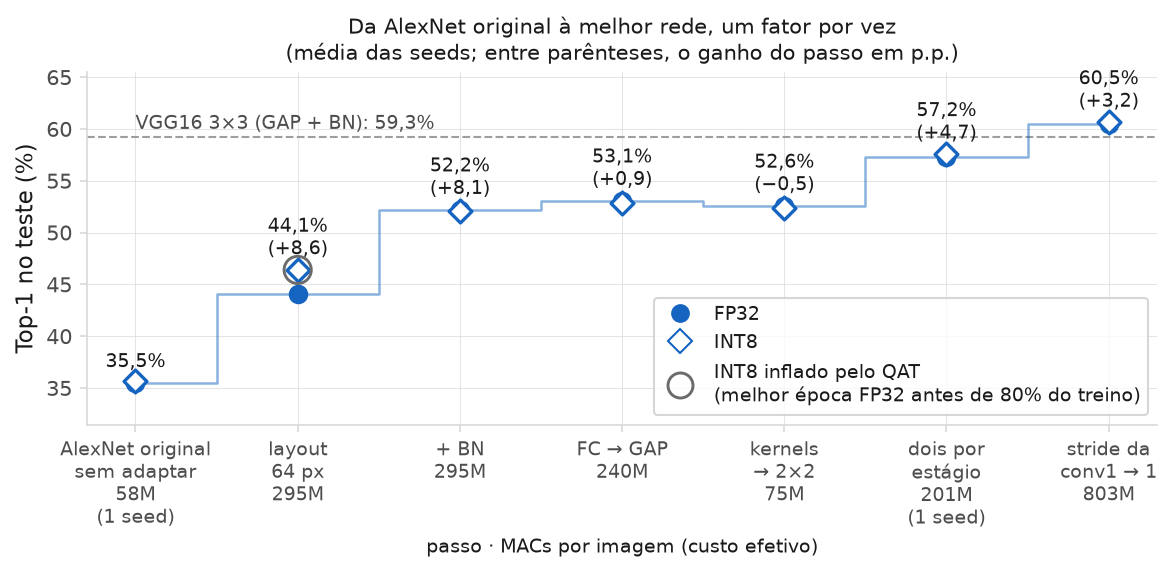
\includegraphics[width=0.78\textwidth,trim=0 0 0 32.2,clip]{phase_13_hybrids/02_caminho.png}
  \nota{Um fator por vez a partir da AlexNet (layout 64 px = strides e poolings ajustados a imagens 64\by64). A melhor rede usa só kernels 2\by2 e supera a VGG16 com 1/6 dos parâmetros (2,3M vs.\ 14,8M).}
\end{frame}

\begin{frame}{INT8 Não Muda a Acurácia}
  \centering
  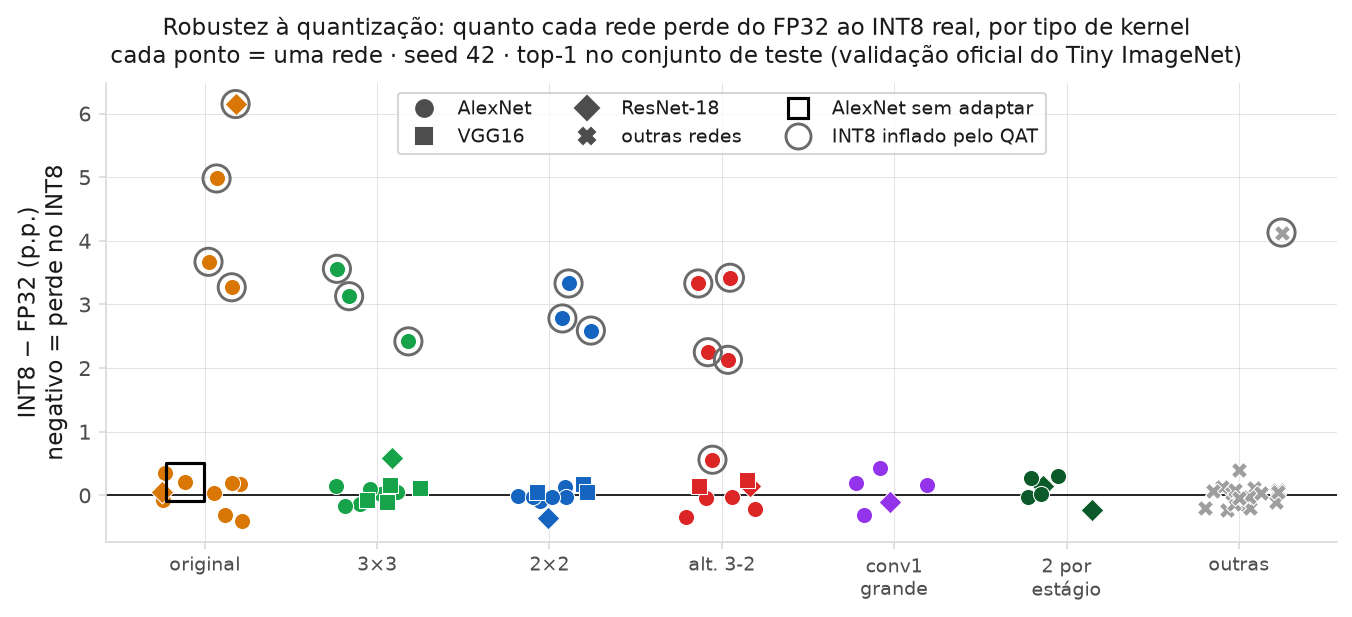
\includegraphics[width=0.92\textwidth,trim=0 0 0 36,clip]{phase_11_kernel_size_comparison/16_quantization_robustness.png}
  \nota{Cada ponto é uma rede. Sem anel, todas ficam perto de zero (mediana $+$0,04 p.p.\ em 140 treinos), seja qual for o kernel. Com anel: a rede ainda melhorava no fim do FP32, e o QAT funcionou como treino extra.}
\end{frame}

\begin{frame}{Winograd no Acelerador}
  \centering
  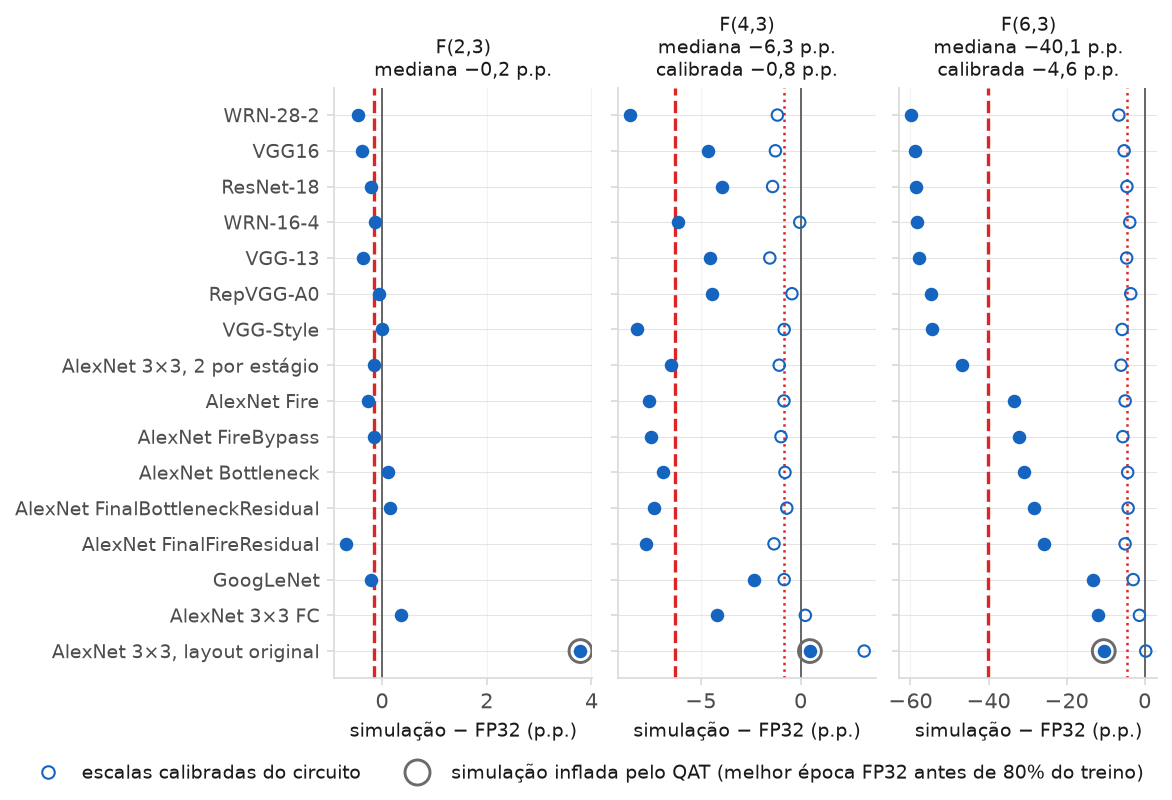
\includegraphics[height=0.65\textheight]{phase_14_winograd_numerics/01_winograd_numerics.png}
  \nota{Cada linha é uma rede. Círculos vazados: escalas do ponto fixo calibradas. Sem calibrar, o F(6,3) leva redes profundas ao acaso.}
\end{frame}

\begin{frame}{Conclusões}
  \begin{itemize}\setlength{\itemsep}{0.6em}
    \item Com cabeça GAP, kernels 2\by2 e 3\by3 custam pouca acurácia e cortam muitos MACs
    \item O que mais pesa é o resto da rede: stride da primeira conv e duas convs por estágio recuperam a perda
    \item Uma rede só com 2\by2 chega a 60,5\,\%, acima da VGG16 (59,3\,\%)
    \item INT8 é de graça; no acelerador, F(2,3) também. Tiles maiores precisam de escalas calibradas
  \end{itemize}
  \bigskip
  \textbf{Próximos passos:} entender por que o erro do F(6,3) se acumula (teste em andamento) e submeter o artigo.
\end{frame}

\begin{frame}{Referências}
  \tiny
  \begin{columns}[T]
    \begin{column}{0.48\textwidth}
      \begin{thebibliography}{10}
        \bibitem{lavin} LAVIN, A.; GRAY, S. Fast algorithms for convolutional neural networks. In: IEEE CVPR, 2016, Las Vegas. \textit{Anais [...]}. Piscataway: IEEE, 2016. p. 4013-4021.
        \bibitem{alexnet} KRIZHEVSKY, A.; SUTSKEVER, I.; HINTON, G. E. ImageNet classification with deep convolutional neural networks. In: NeurIPS, 25., 2012, Lake Tahoe. \textit{Anais [...]}. [S. l.]: Curran Associates, 2012. p. 1097-1105.
        \bibitem{vgg} SIMONYAN, K.; ZISSERMAN, A. Very deep convolutional networks for large-scale image recognition. In: ICLR, 3., 2015, San Diego. \textit{Anais [...]}. [S. l.: s. n.], 2015.
        \bibitem{resnet} HE, K. \textit{et al.} Deep residual learning for image recognition. In: IEEE CVPR, 2016, Las Vegas. \textit{Anais [...]}. Piscataway: IEEE, 2016. p. 770-778.
        \bibitem{squeezenet} IANDOLA, F. N. \textit{et al.} \textit{SqueezeNet: AlexNet-level accuracy with 50x fewer parameters and $<$0.5MB model size}. [S. l.]: arXiv, 2016. arXiv:1602.07360.
      \end{thebibliography}
    \end{column}
    \begin{column}{0.48\textwidth}
      \begin{thebibliography}{10}
        \setcounter{enumiv}{5}
        \bibitem{tiny} LE, Y.; YANG, X. \textit{Tiny ImageNet visual recognition challenge}. Stanford: Stanford University, 2015. (CS231N Course Technical Report).
        \bibitem{jacob} JACOB, B. \textit{et al.} Quantization and training of neural networks for efficient integer-arithmetic-only inference. In: IEEE CVPR, 2018, Salt Lake City. \textit{Anais [...]}. Piscataway: IEEE, 2018. p. 2704-2713.
        \bibitem{wu} WU, H. \textit{et al.} \textit{Integer quantization for deep learning inference: principles and empirical evaluation}. [S. l.]: arXiv, 2020. arXiv:2004.09602.
        \bibitem{barabasz} BARABASZ, B. \textit{et al.} Error analysis and improving the accuracy of Winograd convolution for deep neural networks. \textit{ACM Transactions on Mathematical Software}, v. 46, n. 4, art. 37, 2020.
        \bibitem{schmitz} SCHMITZ, T. H. \textit{et al.} A multi-core Winograd F(2,3) FPGA accelerator with low on-chip memory footprint for VGG16 convolution. In: SBCCI, 2026. \textit{Anais [...]}. 2026.
      \end{thebibliography}
    \end{column}
  \end{columns}
\end{frame}

\begin{frame}[plain]
  \centering\vfill
  {\usebeamerfont{title}\usebeamercolor[fg]{title}Obrigado}
  \vfill
\end{frame}

\end{document}
